%%   $ sudo apt-get install texinfo
%%   $ texi2pdf -c lecture.tex

\PassOptionsToPackage{table}{xcolor}
\documentclass[pdf]{beamer}
\mode<presentation>{\usetheme{Dresden}}
\usepackage{lmodern}
\usepackage{amsmath,textcomp,amssymb,geometry,graphicx,listings,array,color,amsthm}

\usepackage{tikz}
\usepackage{multicol}
\usetikzlibrary{shapes,snakes}
\usetikzlibrary{positioning}
\usetikzlibrary{arrows}
\usetikzlibrary{fit}

%% For on-slide alerting of nodes
\tikzstyle{alert} = [text=black, fill=blue!20, draw=black]
\setbeamercolor{alerted text}{fg=blue}
\tikzset{alerton/.code args={<#1>}{%
  \only<#1>{\pgfkeysalso{alert}} % \pgfkeysalso doesn't change the path
}}

%% utils for removing uninteresting sections from the navbar
%% https://tex.stackexchange.com/questions/317774/hide-section-from-sidebar
\makeatletter
\let\beamer@writeslidentry@miniframeson=\beamer@writeslidentry%
\def\beamer@writeslidentry@miniframesoff{%
  \expandafter\beamer@ifempty\expandafter{\beamer@framestartpage}{}% does not happen normally
  {%else
    % removed \addtocontents commands
    \clearpage\beamer@notesactions%
  }
}
\newcommand*{\miniframeson}{\let\beamer@writeslidentry=\beamer@writeslidentry@miniframeson}
\newcommand*{\miniframesoff}{\let\beamer@writeslidentry=\beamer@writeslidentry@miniframesoff}
\makeatother

%% preamble
\title{BB84}
\subtitle{Quantum \emph{Protected} Cryptography}
\author{A.C.}
\date{\today}

\AtBeginSection[]
{
  \miniframesoff
  \begin{frame}{Outline}
  \tableofcontents
  \end{frame}
  \miniframeson
}

\definecolor{darkred}{rgb}{0.7,0,0}
\definecolor{darkgreen}{rgb}{0,0.5,0}
\definecolor{darkblue}{rgb}{0,0,0.5}
\definecolor{darkpurple}{rgb}{0.4, 0.0, 0.4}

%% Code font settings
\lstset{
  showstringspaces=false,
  basicstyle=\scriptsize\ttfamily,
  commentstyle=\color{darkred},
  stringstyle=\color{darkgreen},
  keywordstyle=\bfseries\color{darkpurple},
}

%%%%%%%%%%%%%%%%%%%%%%%%%%
% Start of Actual slides %
%%%%%%%%%%%%%%%%%%%%%%%%%%
\begin{document}
\begin{frame}
  \titlepage
\end{frame}

\section{Textbook BB84}
\subsection{Quantum Optics Refresher}
\begin{frame}{EM Waves}
  \begin{itemize}
  \item Light is paired waves in electric and magnetic fields
  \pause\item General wave equation \[\nabla^2\Psi = \frac{\partial^2\Psi}{\partial t} \]
  \pause\item Maxwell's equations
    \[ \oint_A E dA = \oint_A B dA = 0 \]
    \[ \oint_C E dl = - \int_A \frac{\partial B}{\partial t} dA\]
    \[ \oint_C B dl = \mu_0 \epsilon \int_A \frac{\partial E}{\partial t} dA \]
  \end{itemize}
\end{frame}
\begin{frame}{Linearly Polarized Light}
  \begin{itemize}
  \item Useful simplified model: assume harmonic, planar waves.
    \begin{itemize}
    \item Between Fourier transforms and other superpositions this covers a
      surprising amount of ground.
    \item Call the orientation of the $E$-wave the light's \emph{polarization}
    \end{itemize}
    \begin{center}
      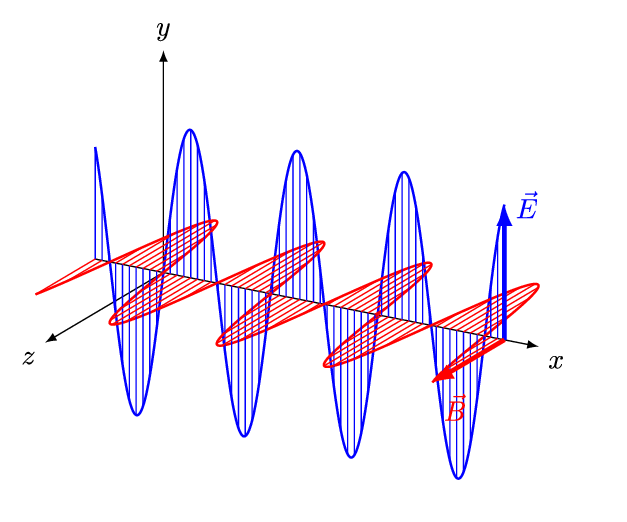
\includegraphics[scale=0.25]{images/EM-Wave.png}
    \end{center}
  \end{itemize}
\end{frame}
\begin{frame}{Polarizers}
  \begin{itemize}
  \item It is possible to create materials which filter light according to its
    polarization
  \pause\item All light passing through a polarizer is dimmed according to the
    alignment of its polarization with the polarizer.
  \pause\item Ideal polarizers follow Malus's law: $I = I_0 cos^2 \theta$
    \begin{center}
      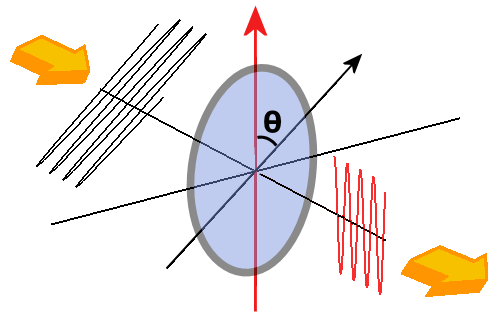
\includegraphics[scale=0.25]{images/Loi_de_malus.png}
    \end{center}
  \end{itemize}
\end{frame}
\begin{frame}{Quantizing}
  \begin{itemize}
  \item EM radiation is transmitted in quanta called \emph{photons}
  \pause\item Still have a polarization due to their wave aspect
    \begin{itemize}
    \item or possibly a superposition of different polarizations \ldots
    \end{itemize}
  \pause\item Cannot be dimmed -- quanta are indivisible.
  \pause\item Instead polarizers absorb with probability $\sin^2\theta$
    \begin{itemize}
    \item or transmit with probability $\cos^2\theta$
    \end{itemize}
  \end{itemize}
\end{frame}
\begin{frame}{No Cloning Theorem}
  \begin{itemize}
  \item Observing a quantum entity, including photons, collapses it into a
    single state.
  \pause\item Impossible to perfectly capture and reconstruct a photon of
    unknown polarization
    \begin{itemize}
    \item Approximate cloning \emph{is} possible, e.g. via stimulated emission
    \item General upper bound on cloning fidelity of $\frac{5}{6}$
    \item Fidelity bound for the case we'll care about of $\approx 0.8535$
    \end{itemize}
  \end{itemize}
\end{frame}

\subsection{BB84}
\begin{frame}{Qubit Bases}
  \begin{itemize}
  \item Photon measurement is deterministic at $\theta=0$ and $\theta=\frac{\pi}{2}$
  \pause\item Map vertically aligned light to $|1\rangle$, horizontally to $|0\rangle$
    \begin{itemize}
    \item Verticality is purely convention
    \item Call the decision of which way is up our \emph{measurement basis}
    \end{itemize}
  \pause\item What happens if sender and receiver use different bases?
    \begin{itemize}
    \item i.e., there's a phase offset of $\phi$ between their verticals
    \end{itemize}
  \pause\item Bit flip with probability $\sin^2 \phi$, by Malus' law.
  \end{itemize}
\end{frame}

\begin{frame}{The Protocol}
  \begin{enumerate}
  \item Alice and Bob publicly agree on two bases (rect, diag) with a
    $\frac{\pi}{4}$ offset between them
  \pause\item Alice creates a random sequence of bits
  \pause\item Alice randomly rect- or diag-encodes each bit, transmits to Bob
  \pause\item Bob randomly rect- or diag-decodes each photon
  \pause\item Alice and Bob publicly announce their basis choices, drop bits where
their bases disagree.
  \pause\item Alice and Bob publicly compare a random subset of the undropped bits.
  \pause\item If they observe a high rate of corruption, they start over.
  \pause\item Otherwise, the undropped and unannounced bits are now a shared secret.
  \end{enumerate}
\end{frame}

\begin{frame}{Protocol in Pictures}
  \begin{center}
    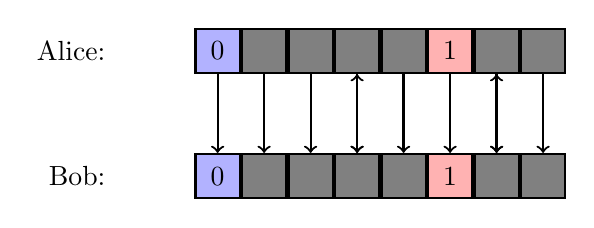
\begin{tikzpicture}[thick,auto,->,minimum size=16pt]
      \uncover<1->{
        \node (a0)[draw=black,fill=blue!30] {0};
        \node[right = 0pt of a0] (a1)[draw=black,fill=red!30] {0};
        \node[right = 0pt of a1] (a2)[draw=black,fill=blue!30] {1};
        \node[right = 0pt of a2] (a3)[draw=black,fill=blue!30] {1};
        \node[right = 0pt of a3] (a4)[draw=black,fill=blue!30] {0};
        \node[right = 0pt of a4] (a5)[draw=black,fill=red!30] {1};
        \node[right = 0pt of a5] (a6)[draw=black,fill=blue!30] {0};
        \node[right = 0pt of a6] (a7)[draw=black,fill=red!30] {1};

        \node[left = of a0] (alice) {Alice:};
      }
      \uncover<2->{
        \node[below = of a0] (b0)[draw=black,fill=blue!30] {?};
        \node[below = of a1] (b1)[draw=black,fill=blue!30] {?};
        \node[below = of a2] (b2)[draw=black,fill=red!30]  {?};
        \node[below = of a3] (b3)[draw=black,fill=blue!30] {?};
        \node[below = of a4] (b4)[draw=black,fill=red!30]  {?};
        \node[below = of a5] (b5)[draw=black,fill=red!30]  {?};
        \node[below = of a6] (b6)[draw=black,fill=blue!30] {?};
        \node[below = of a7] (b7)[draw=black,fill=blue!30] {?};

        \node[left = of b0] (bob) {Bob:};
      }
      \uncover<3->{
        \node[below = of a0] (b0f)[draw=black,fill=blue!30] {0};}
      \uncover<4->{
        \node[below = of a1] (b1f)[draw=black,fill=blue!30] {0};}
      \uncover<5->{
        \node[below = of a2] (b2f)[draw=black,fill=red!30]  {0};}
      \uncover<6->{
        \node[below = of a3] (b3f)[draw=black,fill=blue!30] {1};
        \node[below = of a4] (b4f)[draw=black,fill=red!30]  {1};
        \node[below = of a5] (b5f)[draw=black,fill=red!30]  {1};
        \node[below = of a6] (b6f)[draw=black,fill=blue!30] {0};
        \node[below = of a7] (b7f)[draw=black,fill=blue!30] {1};}
      \uncover<7->{
        \node[right = 0pt of a0] (a1r)[draw=black,fill=gray] {};
        \node[right = 0pt of a1] (a2r)[draw=black,fill=gray]  {};
        \node[right = 0pt of a3] (a4r)[draw=black,fill=gray]  {};
        \node[right = 0pt of a6] (a7r)[draw=black,fill=gray] {};
        \node[below = of a1] (b1r)[draw=black,fill=gray] {};
        \node[below = of a2] (b2r)[draw=black,fill=gray]  {};
        \node[below = of a4] (b4r)[draw=black,fill=gray]  {};
        \node[below = of a7] (b7r)[draw=black,fill=gray] {};
      }
      \uncover<9->{
        \node[right = 0pt of a2] (a3r)[draw=black,fill=gray]  {};
        \node[right = 0pt of a5] (a6r)[draw=black,fill=gray] {};
        \node[below = of a3] (b3r)[draw=black,fill=gray]  {};
        \node[below = of a6] (b6r)[draw=black,fill=gray] {};
      }

      \uncover<3>{
        \path (a0) edge (b0);}
      \uncover<4>{
        \path (a1) edge (b1);}
      \uncover<5>{
        \path (a2) edge (b2);}
      \uncover<6>{
        \path (a3) edge (b3);
        \path (a4) edge (b4);
        \path (a5) edge (b5);
        \path (a6) edge (b6);
        \path (a7) edge (b7);
      }
      \uncover<8>{
        \path (a3) edge[<->] (b3);
        \path (a6) edge[<->] (b6);
      }
    \end{tikzpicture}
  \end{center}
  \vspace{10pt}
  \only<1>{Alice selects random bits, bases}
  \only<2>{Bob selects random bases}
  \only<3>{Bases agree, measurement succeeds}
  \only<4-5>{Bases disagree, measurement \emph{may} fail}
  \only<6>{Etc...}
  \only<7>{Sift out mismatched bases}
  \only<8>{Sample bits to detect Eve}
  \only<9>{Redact sampled bits}
\end{frame}

\begin{frame}{BB84 Intuition}
  \begin{itemize}
  \item Rectilinear and diagonal bases chosen to maximize corruption
    \begin{itemize}
    \item Decoding in the wrong basis yields a $50\%$ chance of corruption.
    \end{itemize}
  \pause\item If Eve intercepts a photon and forwards it on to Bob, she'll likely
    corrupt it.
    \begin{itemize}
    \item $50\%$ chance she's in the wrong basis
    \item $50\%$ chance of corruption from mis-encoding.
    \item $25\%$ Bob gets a corrupted bit (assuming no intelligent cloning).
    \end{itemize}
  \pause\item Can't stop Eve, but can \emph{detect} her.
  \end{itemize}
\end{frame}

\section{Textbook to Production}
\subsection{Error Correction}
\begin{frame}{Benign QBER}
  \begin{itemize}
  \item Sending and receiving individual quanta is \emph{hard}
  \pause\item Even if Eve isn't interfering, some of our bits will be scrambled.
  \pause\item Secrets which are mostly the same are not nearly as useful as secrets which are
    exactly the same.
  \pause\item We need to somehow rectify the differences between what Alice sent and
    Bob received.
  \end{itemize}
\end{frame}
\begin{frame}{Single Error Detection}
  \begin{itemize}
  \item Start with 4 data bits $d_1,d_2,d_3,d_4$.
    \begin{itemize}
    \item How can we detect a lone bit flip?
    \end{itemize}
  \pause\item Idea, add parity bit at the end: $p_1 := d_1 \oplus d_2 \oplus d_3 \oplus d_4$
  \pause\item If we retrieve our code word $(d_1,d_2,d_3,d_4,p_1)^T$ in the future and
    it has odd parity, at least one bit must have been flipped.
  \pause\item Can write as a check matrix: \[ H = \begin{pmatrix}
        1 & 1 & 1 & 1 & 1
      \end{pmatrix} \]
  \end{itemize}
\end{frame}
\begin{frame}{Single Error Correction}
  \begin{itemize}
    \item If we want to correct an error, we need to know \emph{which} bit was
      flipped.
    \pause\item Let's add more parity bits, but
      \begin{itemize}
      \item Each parity bit will only cover some bits in the code word.
      \item We'll be careful to make sure that every bit is covered by a unique
        combination of parity bits
      \end{itemize}
    \pause\item Hamming solved this for us in 1950 using powers of two
      \begin{itemize}
      \item Code word: $(p_1,p_2,d_1,p_3,d_2,d_3,d_4)^T$
      \item Check matrix: \[ H = \begin{pmatrix}
            1 & 0 & 1 & 0 & 1 & 0 & 1 \\
            0 & 1 & 1 & 0 & 0 & 1 & 1 \\
            0 & 0 & 0 & 1 & 1 & 1 & 1
          \end{pmatrix} \]
      \end{itemize}
  \end{itemize}
\end{frame}
\begin{frame}{Full SECDED}
  \begin{itemize}
  \item Glue a total parity bit onto a Hamming SEC scheme
    \begin{itemize}
    \item No errors $\implies$ all parity checks report even
    \item Single error $\implies$ total parity reports odd, SEC parities indicate location
    \item Double error $\implies$ total parity reports even, SEC parities indicate ``location''
    \end{itemize}
  \pause\item Commonly known as Hamming(8,4).
    \begin{itemize}
      \item Code word: $(p_1,p_2,d_1,p_3,d_2,d_3,d_4,p_\text{total})^T$
      \item Check matrix: \[ H = \begin{pmatrix}
            1 & 0 & 1 & 0 & 1 & 0 & 1 & 0 \\
            0 & 1 & 1 & 0 & 0 & 1 & 1 & 0 \\
            0 & 0 & 0 & 1 & 1 & 1 & 1 & 0 \\
            1 & 1 & 1 & 1 & 1 & 1 & 1 & 1
          \end{pmatrix} \]
      \end{itemize}
  \end{itemize}
\end{frame}

\begin{frame}{Winnow I}
  \begin{itemize}
  \item What if we just pretended our sifted qubits were SECDED code words?
  \pause\item They're not, so if Alice has a block $a$, then $Ha$ will almost always
    want to ``correct'' something.
    \begin{itemize}
    \item And for Bob, $Hb$ will behave similarly
    \end{itemize}
  \pause\item $a \oplus b \approx 0 \implies H(a \oplus b) = Ha \oplus Hb \approx 0$
  \pause\item What if we compare $Ha$ and $Hb$, have Bob apply SECDED using
    $Ha \oplus Hb$?
    \begin{itemize}
    \item If even errors, do nothing
    \item If odd errors, probably $d(a, b') = d(a, b) - 1$
    \end{itemize}
  \pause\item We can reconcile errors by exchanging Hamming syndromes!
  \end{itemize}
\end{frame}
\begin{frame}{Winnow II}
  \begin{enumerate}
  \item Alice and Bob break their bits into SECDED code words
  \pause\item Alice and Bob exchange total parity for each codeword
    \begin{enumerate}
    \item blocks whose total parities agree are ignored going forward
    \end{enumerate}
  \pause\item Alice sends Bob $Ha$ for each remaining block
  \pause\item Bob applies SEC using $Ha \oplus Hb$
  \pause\item Alice and Bob discard all announced parity bits
    \begin{enumerate}
    \item Keeps Eve from gleaning info from our error correction process.
    \end{enumerate}
  \pause\item Alice and Bob shuffle their remaining bits using the same seed.
    \begin{enumerate}
    \item Stops an even number of errors from ``sticking'' in a code word.
    \end{enumerate}
  \pause\item Go back to (1) until convinced that the probability of surviving errors
    is negligible.
  \end{enumerate}
\end{frame}

\subsection{Privacy Amplification}
\begin{frame}{Bit Leakage}
  \begin{itemize}
  \item Real systems have some amount of legitimate error
  \pause\item Paranoia requires that we treat all errors as due to eavesdropping
  \pause\item \emph{Eve is allowed to have partial information on our secret!}
    \begin{itemize}
    \item Or we can just never succeed in negotiating a secret
    \end{itemize}
  \pause\item Need to do two things
    \begin{itemize}
    \item Estimate how many bits of information Eve has
    \item Somehow scrub those bits out of our secret
    \end{itemize}
  \end{itemize}
\end{frame}
\begin{frame}{Parameter Estimation I}
  \begin{itemize}
  \item Whenever Eve performs an intercept/resend, she risks creating an error
    \begin{itemize}
    \item $\text{QBER} \sim \frac{1}{n} \cdot \text{Bin}(n, p)$
    \pause\item Theoretical bound of $2 \sqrt{2}$ bits of information per bit flipped (in the long run)
    \pause\item If we can estimate $p$ we can determine how many bits Eve has
    \end{itemize}
  \pause\item Estimate $\hat{p} = \text{QBER}$?
    \begin{itemize}
    \item Too easy to have $\hat{p} < p$
    \end{itemize}
  \pause\item Bayes rule to pick $\hat{p}$ s.t. $P(p > \hat{p} | \text{QBER}) < \epsilon$?
    \begin{itemize}
    \item No sensible prior to put on $p$
    \end{itemize}
  \end{itemize}
\end{frame}
\begin{frame}{Parameter Estimation II}
  \begin{itemize}
  \item Treat $M$, our bits to scrub, as an random variable $f(X)$
  \pause\item If $P(M < 2\sqrt{2} \cdot p) < \epsilon$, we win
    \begin{itemize}
    \item Sounds an awful lot like a confidence interval
    \end{itemize}
  \pause\item Calculating CIs for a binomial distribution on the fly can be cumbersome
    \begin{itemize}
    \item Common to pick $m$, $p_\text{crit}$ in advance
    \item Always trim off $m$ bits, bail if $QBER > p_\text{crit}$
    \end{itemize}
  \end{itemize}
\end{frame}
\begin{frame}{Mopping up the Leak}
  \begin{itemize}
  \item Soooo, can we just hash our secret from $n$ bits down to $m$?
  \pause\item Yes, if we:
    \begin{itemize}
    \item use a universal hash family
    \item trim an additional $2 \log \left( \frac{1}{\epsilon} \right)$ bits
    \item choose our hash function randomly, although it \emph{can} be public
    \end{itemize}
  \pause\item This is a direct result of the
    \underline{\href{https://www.cs.bu.edu/~reyzin/teaching/s11cs937/notes-leo-1.pdf}{leftover
        hash lemma}}
  \pause\item Approach is obvious:
    \begin{enumerate}
    \item Alice publicly announces a random seed
    \item Alice and Bob both use the seed to hash their secrets down
    \end{enumerate}
  \end{itemize}
\end{frame}

\subsection{Authentication}
\begin{frame}{MITM}
  \begin{itemize}
  \item Trivial attack: Eve plops herself between Alice and Bob
  \pause\item Alice and Bob wind up with different secrets, but Eve knows
    both and they only ever talk to her.
  \pause\item Need some sort of authentication scheme
    \begin{itemize}
    \item Impossible without some sort of bootstrap secret!
    \item But we can still use the scheme to stretch the bootstrap secret,
      e.g. to allow for one-time pads in the data plane.
    \end{itemize}
  \pause\item Our goal is unconditional security, so a standard HMAC won't cut it.
  \end{itemize}
\end{frame}
\begin{frame}{One Time MAC}
  \begin{enumerate}
  \item Use $l$ bits of bootstrap secret to choose a member of a universal hash
    family.
  \pause\item Hash the message to authenticated into an $m$-bit message tag.
  \pause\item Encrypt the tag with a one-time pad.
  \pause\item Discard the $m$ bits used for the OTP.
  \end{enumerate}
\end{frame}
\begin{frame}{One Time MAC Intuitions}
  \begin{itemize}
  \item Eve can't manufacture a hashes for messages, doesn't know
    the hash function.
    \begin{itemize}
    \item Otherwise, she could backward engineer the pad used to encrypt legitimate MACs
    \end{itemize}
  \pause\item The hash value is encrypted, so she can't manufacture a hash collision.
    \begin{itemize}
    \item Universal hash function means she can't even make intelligent guesses
      about the hash value.
    \end{itemize}
  \pause\item Best she can do is guess the tag
    \begin{itemize}
    \item Succeeds with probability $\frac{1}{2^m}$
    \item Places a tradeoff between key expenditure and probability that Eve
      gets lucky.
    \end{itemize}
  \end{itemize}
\end{frame}

\subsection{Photon Number Splitting}
\begin{frame}{PNS}
  \begin{itemize}
  \item Emitting a single photon is bloody hard
  \pause\item Most experimental setups work by dimming a laser pulse down to
    $\approx 1$ photon
    \begin{itemize}
    \item Possible for a pulse to include multiple photons.
    \end{itemize}
  \pause\item Eve could sniff multi-photon pulses without corrupting them
  \pause\item Can also block single-photon pulses to stop Alice/Bob from using them
    in the secret.
    \begin{itemize}
    \item Bob expects a lot of transmissions to get lost, this won't necessarily
      set off alarm bells
    \end{itemize}
  \pause\item Attack is commonly known as photon number splitting
  \end{itemize}
\end{frame}
\begin{frame}{Decoy States}
  \begin{itemize}
  \item Alice uses two (or more) signal sources $S$ and $S'$
    \begin{itemize}
    \item $S$ is the real photon source, averages $\mu$ photons per pulse
    \item $S'$ is a decoy, with $\mu' > \mu$
    \item Upshot: $S$ sends more single photon pulses than $S'$
    \end{itemize}
  \pause\item Impossible for Eve to tell whether a given pulse came from $S$ or $S'$
  \pause\item By blocking single photon pulses, Eve will affect the transmission rate
    for $S$ more than for $S'$.
  \pause\item Alice and Bob can compare empirical transmission loss for $S$ and $S'$
    at the end.
    \begin{itemize}
    \item If they differ, they conclude Eve did something naughty.
    \end{itemize}
  \end{itemize}
\end{frame}

%% Q&A and Further reading.
\miniframesoff
\section*{}
\begin{frame}{TL;DR}
  \begin{enumerate}
  \item Send/receive a stream of quanta in random bases.
  \item Throw away the bits where bases disagreed.
  \item Reconcile keys using (adaptations of) standard error correction schemes.
  \item Hash your keys down according to pessimistic estimates of how much
    information Eve could have.
  \item Make sure to authenticate all your messages throughout.
  \item Profit!
  \end{enumerate}
\end{frame}

\begin{frame}{References and Additional Materials}
  \begin{itemize}
  \item Presentation source:
    \url{https://github.com/alan-christopher/bb84/tree/master/edu}
  \item Quantum Cryptography Intro: \url{https://arxiv.org/abs/1002.1237}
  \item Quantum Cloning: \url{https://arxiv.org/abs/quant-ph/0511088}
  \item Privacy Amplification: \url{https://link.springer.com/article/10.1007/BF00191318}
  \item Winnow: \url{https://arxiv.org/abs/quant-ph/0203096}
  \item Decoy states: \url{https://arxiv.org/abs/quant-ph/0211153} % \url{https://arxiv.org/abs/quant-ph/0411004}
  \item A QKD implementation: \url{https://arxiv.org/abs/1603.08387}
  \end{itemize}
\end{frame}

\begin{frame}{Included Works}
  \begin{itemize}
  \item \underline{\href{https://commons.wikimedia.org/wiki/File:EM-Wave.gif}{Transverse Wave Image}}
  \item \underline{\href{https://commons.wikimedia.org/wiki/File:Loi_de_malus.png}{Polarizer Image}}
  \end{itemize}
\end{frame}

\begin{frame}{Questions?}
\end{frame}
\end{document}
